% Targeted build: pdflatex -output-directory=<build> net-twist-reduction.tex
% SVG and PNG are direct exports of the resulting PDF page.
\documentclass[tikz,border=12pt]{standalone}
\usepackage[T1]{fontenc}
\usepackage{lmodern,amsmath}
\usetikzlibrary{arrows.meta}
\definecolor{ink}{HTML}{183444}
\definecolor{blue}{HTML}{1B6780}
\definecolor{amber}{HTML}{AD601A}
\newcommand{\tanglebox}[4]{%
  \draw[draw=#4,fill=#4!6,rounded corners=2pt]
    (#1-.9,#2-.6) rectangle (#1+.9,#2+.6);
  \node[font=\large] at (#1,#2) {$#3$};
}
\newcommand{\stackstrands}[1]{%
  \foreach \dx in {-.55,.55}{
    \draw[blue] (#1+\dx,-4.75)--(#1+\dx,-4.2);
    \draw[blue] (#1+\dx,-3.0)--(#1+\dx,-2.0);
    \draw[blue] (#1+\dx,-.8)--(#1+\dx,-.25);
    \fill[blue] (#1+\dx,-4.75) circle (1.6pt);
    \fill[blue] (#1+\dx,-.25) circle (1.6pt);
  }
  \node[font=\scriptsize,below] at (#1-.55,-4.75) {$0$};
  \node[font=\scriptsize,below] at (#1+.55,-4.75) {$1$};
  \node[font=\scriptsize,above] at (#1+.55,-.25) {$2$};
  \node[font=\scriptsize,above] at (#1-.55,-.25) {$3$};
}
\begin{document}
\hyphenpenalty=10000\exhyphenpenalty=10000
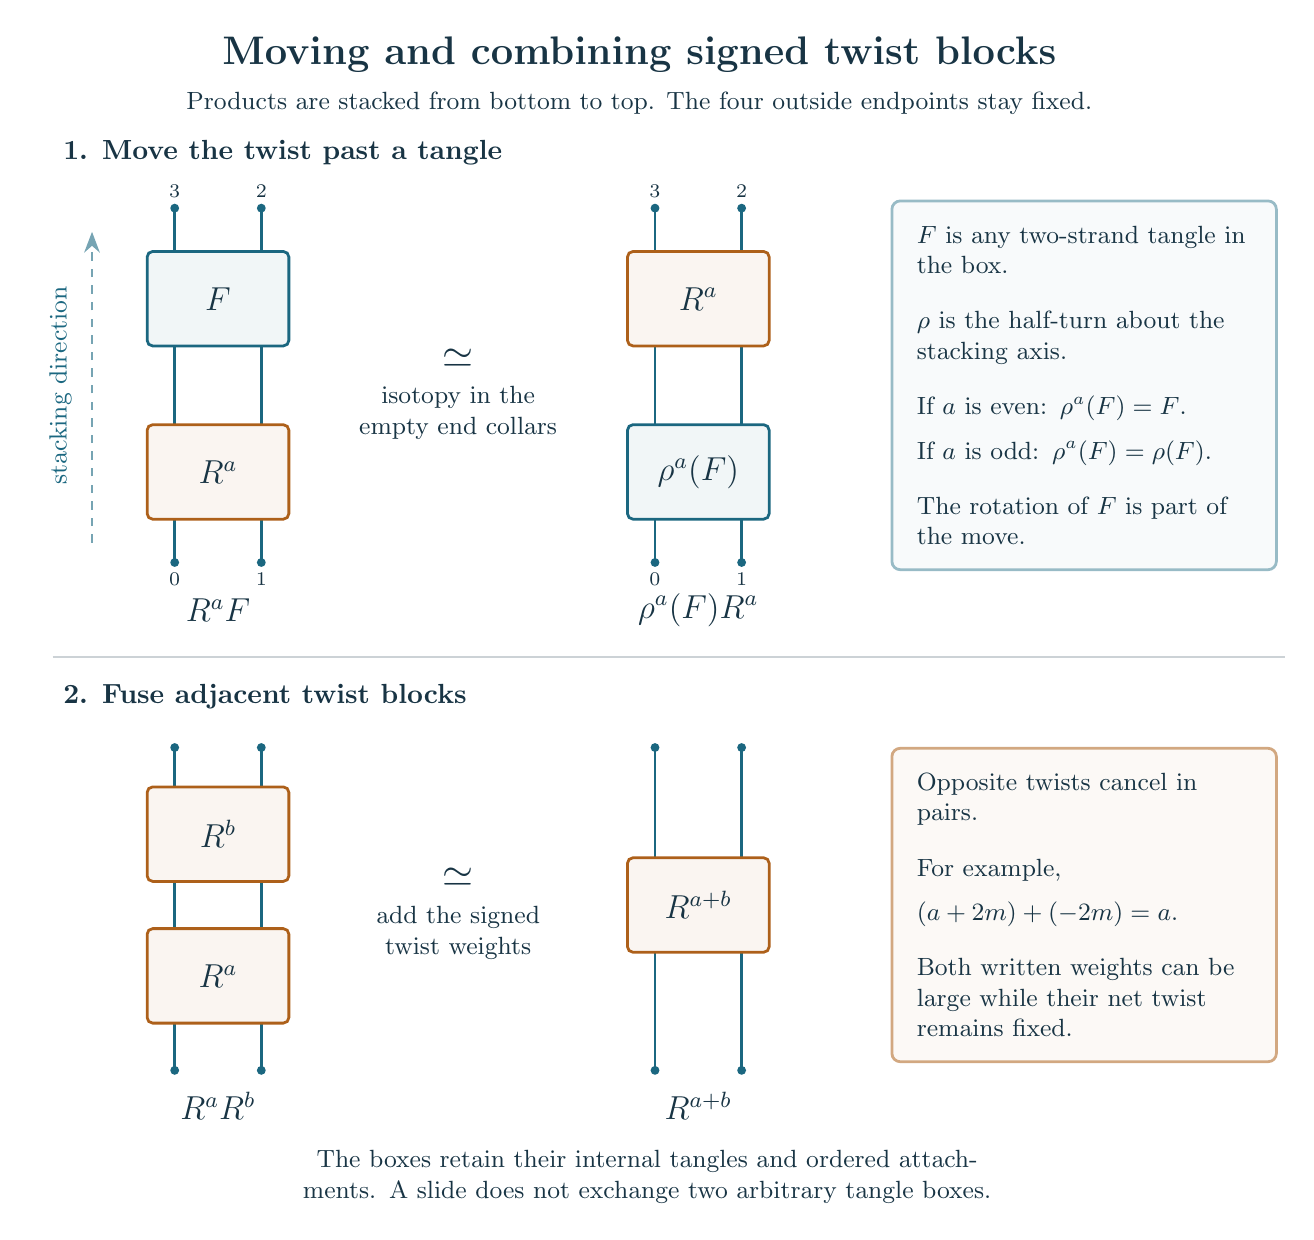
\begin{tikzpicture}[font=\sffamily,text=ink,line width=1pt,>=Stealth,
  explanation/.style={draw=blue!45,fill=blue!3,rounded corners=3pt,
    text width=4.25cm,align=left,inner sep=9pt,font=\small}]
  \node[font=\Large\bfseries] at (7.5,1.7)
    {Moving and combining signed twist blocks};
  \node[font=\small,align=center] at (7.5,1.08)
    {Products are stacked from bottom to top. The four outside endpoints stay fixed.};

  \node[anchor=west,font=\bfseries] at (.05,.45) {1. Move the twist past a tangle};
  \stackstrands{2.15}
  \tanglebox{2.15}{-3.6}{R^a}{amber}
  \tanglebox{2.15}{-1.4}{F}{blue}
  \stackstrands{8.25}
  \tanglebox{8.25}{-3.6}{\rho^a(F)}{blue}
  \tanglebox{8.25}{-1.4}{R^a}{amber}
  \draw[blue!60,dashed,->] (.55,-4.5)--(.55,-.55);
  \node[rotate=90,font=\small,text=blue] at (.15,-2.5) {stacking direction};
  \node[font=\Large] at (5.2,-2.15) {$\simeq$};
  \node[font=\small,align=center,text width=2.6cm] at (5.2,-2.85)
    {isotopy in the\\empty end collars};
  \node[font=\large] at (2.15,-5.35) {$R^aF$};
  \node[font=\large] at (8.25,-5.35) {$\rho^a(F)R^a$};
  \node[explanation] at (13.15,-2.5) {
    $F$ is any two-strand tangle in the box.\\[9pt]
    $\rho$ is the half-turn about the stacking axis.\\[9pt]
    If $a$ is even: $\rho^a(F)=F$.\\[5pt]
    If $a$ is odd: $\rho^a(F)=\rho(F)$.\\[9pt]
    The rotation of $F$ is part of the move.};

  \draw[ink!22] (.05,-5.95)--(15.7,-5.95);
  \node[anchor=west,font=\bfseries] at (.05,-6.45) {2. Fuse adjacent twist blocks};
  \begin{scope}[yshift=-7.5cm]
    \foreach \dx in {-.55,.55}{
      \draw[blue] (2.15+\dx,-3.7)--(2.15+\dx,-3.1);
      \draw[blue] (2.15+\dx,-1.9)--(2.15+\dx,-1.3);
      \draw[blue] (2.15+\dx,-.1)--(2.15+\dx,.4);
      \fill[blue] (2.15+\dx,-3.7) circle (1.6pt);
      \fill[blue] (2.15+\dx,.4) circle (1.6pt);
      \draw[blue] (8.25+\dx,-3.7)--(8.25+\dx,-2.2);
      \draw[blue] (8.25+\dx,-1.0)--(8.25+\dx,.4);
      \fill[blue] (8.25+\dx,-3.7) circle (1.6pt);
      \fill[blue] (8.25+\dx,.4) circle (1.6pt);
    }
    \tanglebox{2.15}{-2.5}{R^a}{amber}
    \tanglebox{2.15}{-.7}{R^b}{amber}
    \tanglebox{8.25}{-1.6}{R^{a+b}}{amber}
    \node[font=\Large] at (5.2,-1.25) {$\simeq$};
    \node[font=\small,align=center,text width=2.8cm] at (5.2,-1.95)
      {add the signed\\twist weights};
    \node[font=\large] at (2.15,-4.15) {$R^aR^b$};
    \node[font=\large] at (8.25,-4.15) {$R^{a+b}$};
    \node[explanation,draw=amber!55,fill=amber!4] at (13.15,-1.6) {
      Opposite twists cancel in pairs.\\[9pt]
      For example,\\[5pt]
      $\displaystyle(a+2m)+(-2m)=a$.\\[9pt]
      Both written weights can be large while their net twist remains fixed.};
  \end{scope}
  \node[font=\small,align=center,text width=15.5cm] at (7.6,-12.55)
    {The boxes retain their internal tangles and ordered attachments. A slide does not exchange two arbitrary tangle boxes.};
\end{tikzpicture}
\end{document}
